% !Mode:: "TeX:UTF-8"
%!TEX program  = xelatex

\documentclass[bwprint]{cumcmthesis}
%\documentclass[withoutpreface,bwprint]{cumcmthesis} %去掉封面与编号页

\title{优化汽车后视镜设计}
\tihao{A}
\baominghao{201723003xxx}
\schoolname{电子科技大学}
\membera{卫佳杰}
\memberb{谢沁余}
\memberc{任彦璟}
\supervisor{覃思义}
\yearinput{2017}
\monthinput{07}
\dayinput{13}

\begin{document}
 \maketitle
 \begin{abstract}
 \par 汽车的后视镜需要有良好的视野范围使驾驶员能够全面地了解汽车后方以及两侧的道路情况,同时也要保证在后视镜中看到图像的畸变尽可能小使驾驶员能够准确地判断两车距离。本文将给出汽车后视镜的最优设计方案。
\par 本文首先对双曲率外后视镜的模型提出了两种连接方案,方案中两个关键参数为分界线的位置和小球的曲率半径。通过在外后视镜镜面上均匀投点,结合反射定律和人眼位置计算给定距离外的物像。视野范围依据国家标准,即在指定距离后找能看到的最大宽度。本文建立了畸变率计算模型,并验证了平面镜畸变率为0。接着通过计算机模拟的方法,同时改变这分界线位置和小球曲率半径,求解畸变率和视野范围。本文设置指标综合畸变率和视野范围,在两方案中选择出最优方案:大球面镜曲率半径为1260mm,小球面镜曲率半径为500mm,分界线在外后视镜外侧的$1/5$处。
\par 本文给出一种驾驶员通过后视镜中后车图像宽度占后视镜镜长的大致比例来推断两车距离的办法。例如:在左后视镜中,驾驶员最终确定出当后车的图像线段宽度占整个后视镜镜长的$1/2$时,两车的距离约为20米;在右后视镜中,驾驶员最终确定出当后车的图像线段宽度占整个后视镜镜长的$1/2$时,两车的距离约为8米。由于司机对后视镜的中的图像的占比是一个估计值,所以对距离的预估会产生一定的偏差。
\par 本文选择奇瑞QQ车型进行验证,该车型采用的单曲率后视镜,曲率半径为$1200mm$,将该后视镜的参数带入模型得到驾驶员左侧的视野范围为$4553mm$,畸变率为$2.9\%$。右侧的视野范围为$7997mm$,并且此时的畸变率为$10.3\%$。本文设计的双曲率后视镜采取曲率半径分别为$1260mm$与$500mm$,得到驾驶员的左侧视野范围为$5527mm$,畸变率为$3.8\%$;右侧的视野范围为$11536mm$,畸变率为$11.4\%$。对比得到本文在畸变率基本不变的基础上使左右两侧的视野范围大大增加,验证本文的设计优于原设计。
 
\keywords{畸变率  \quad 视野范围  \quad 目标规划 \quad 光学原理 \quad 光学投点}
\end{abstract}

\tableofcontents
\newpage

\section{问题重述}
 

\subsection{引言}

\par 野范围尽可能覆盖汽车的两侧与后方的区域,以便驾驶员能够全面地了解车后方的道路情况。

\par 最常见的是一种双曲率后视镜,内侧接近平面镜,外侧则是一个凸面镜,在它们之间进行了平滑的过渡。为了便于驾驶员对距离进行判断,镜中由虚线或细实线示意了不同曲率的镜面间的分界线(如图(\ref{title})所示)。当然还可以考虑更多曲率以及之间的过渡形式。比如,在侧方位停车时,需要看到后车轮的位置,可能考虑在后视镜下方能有曲率变化。

\begin{figure}[!htb]
\centering
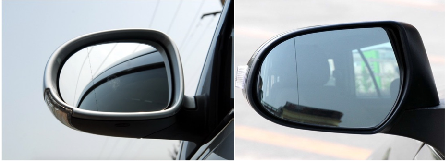
\includegraphics[width=\textwidth]{title.png}
\caption{变曲率后视镜示例}
\label{title}
\end{figure}

\subsection{问题的提出}

围绕优化汽车后视镜的设计、验证过程,本文依次提出如下问题:

\begin{enumerate}
  \item 假设两面外后视镜都设计成双曲率后视镜(或多曲率后视镜),建立相应的数学模型,在后视镜面积一定的条件下,对外后视镜给出优化的设计方案,包括镜面的曲面外形以及分界示意线的位置。
  \item 请就设计的最优后视镜,给出一种方便司机简单易行的快速判断镜中物体的距离与方位的方法。该判别方法要考虑一定的误差。
  \item 以一种现有的轿车为例,镜面的边缘轮廓可以沿用现有的设计的基础上,给出具体的计算结果。 
\end{enumerate}

\section{问题分析}

\par 在国家车辆标准的现有基础上,对左侧后视镜的视野范围定义为驾驶员能看到后视镜后方10米处,距离车身的范围。对右侧后视镜的视野范围定义为驾驶员能看到后视镜后方20米处,距离车身的范围。我们采用畸变率来衡量驾驶员看到的图像与实际图像的偏差。如果汽车的后视镜使用平面镜,图像没有畸变,对距离和方位的判断十分准确。但是当镜面大小受限时,视野相对较小。如果使用凸面镜,可以以较小的镜面获得更加宽广的视野,但是图像存在较大畸变,难以准确判断镜中物体与自己的距离及镜中物体与自己的相对方位。汽车外后视镜的设计需要满足视野尽可能大的同时减少图像的畸变率。

\subsection{问题一}

\par 设计的双曲率外后视镜,首先要确定曲率半径不同下的两球面的球心坐标,通过球心的坐标,确定球面的位置,得到球面方程,通过反射定理,得出双曲率外后视镜的畸变率及左右外后视镜各自的的水平(垂直)视野范围,在畸变率保持在可接受范围内的基础上,使外后视镜的视野范围最大。同时确定出双曲率后视镜两不同曲率的最优分界线。
\subsection{问题二}

\par 在问题一设计的基础上确定驾驶员看到的后方车辆在镜面上的图像的宽度占外后视镜宽度的比例,给出司机简易快速判断后视镜中物体与本车距离、方位的判断方法。收集统计量产车数据得到常见车辆平均宽度数据,经过模型计算得到后视镜中像的大小与后车车距的比例关系,并且分析快速判断方法造成的误差。
\subsection{问题三}

\par 根据选定的量产车的实际数据,计算得到评价模型的各个参数。 

\section{模型的假设}

\begin{enumerate}
	\item 本文设计的双曲率球面外后视镜在分界线两侧保持曲率恒定,忽略过渡处,认为过渡处可用工艺加工变平滑。
	\item 外后视镜安装时遵循其水平中线与人视线在同一水平面上的原则。
	\item 最初按照最小模型($70mm \times 72.48mm$)设计,再对照实际进行等比放大和截取,从而得到最终设计的外后视镜。
	\item 计算视野范围时,司机的眼点依据国家标准。通过汽车制造厂确定的驾驶员设计乘坐位置中心,作一个平行于汽车纵向基准面的平面。从该平面内的驾驶员座椅$R$点向上$635mm$,作垂直于该平面的一条直线段。在直线段与该平面交点的两侧各$32.5mm$处作两个点,即为驾驶员的眼点。
	\item 在计算畸变率时,取眼点连线的中点处作为人眼的位置。
	\item 平均车宽取1700mm。  
\end{enumerate}


\section{符号说明}

\begin{tabular}{cc}
\toprule
 \makebox[0.4\textwidth][c]{符号}	&  \makebox[0.5\textwidth][c]{意义} \\ \midrule
 $\alpha$	    & 畸变率 \\ 
 $K$	    & 综合指标  \\ 
 $L$	    & 水平视野宽度  \\ 
 $Q_1$	    & 主视野区(大曲率半径)镜面球心  \\ 
 $Q_2$	    & 副视野区(小曲率半径)镜面球心  \\ 
 $dis$	    & 光屏距离外后视镜的距离  \\ 

\bottomrule 
\end{tabular}

\section{模型建立}
\subsection{视野范围模型}

\begin{figure}[!htb]
\centering
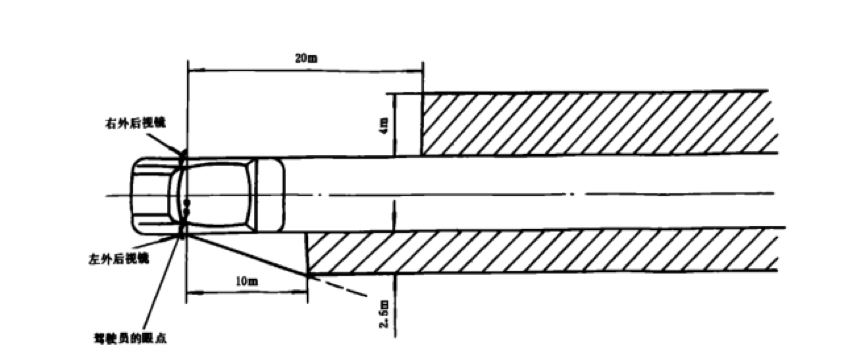
\includegraphics[width=\textwidth]{view.png}
\caption{水平视野范围的定义}
\label{view}
\end{figure}

\par 在司机的最大视野范围模型中,在水平方向上根据国家标准$GB 15084-94$(如图(\ref{view})所示),对左侧后视镜,将距后视镜10米处,司机从后视镜所能观测到的水平宽度定义为左侧水平视野范围。同时根据国家标准$GB 15084-94$,通过调整后视镜的空间方位,驾驶员借助左侧后视镜必须可观测到水平宽度为2.5米的水平视野区域,将该视野范围定义为左侧水平视野范围下限。

\par 同理,对右侧后视镜,将距后视镜20米处,司机从后视镜能观测到的水平宽度定义为右侧水平视野范围,右侧水平视野范围下限为4米。
\par 如图(\ref{hight})所示,将通过后视镜在后车轮处能够观测到的最低垂直高度定义为垂直视野范围。

\begin{figure}[!htb]
\centering
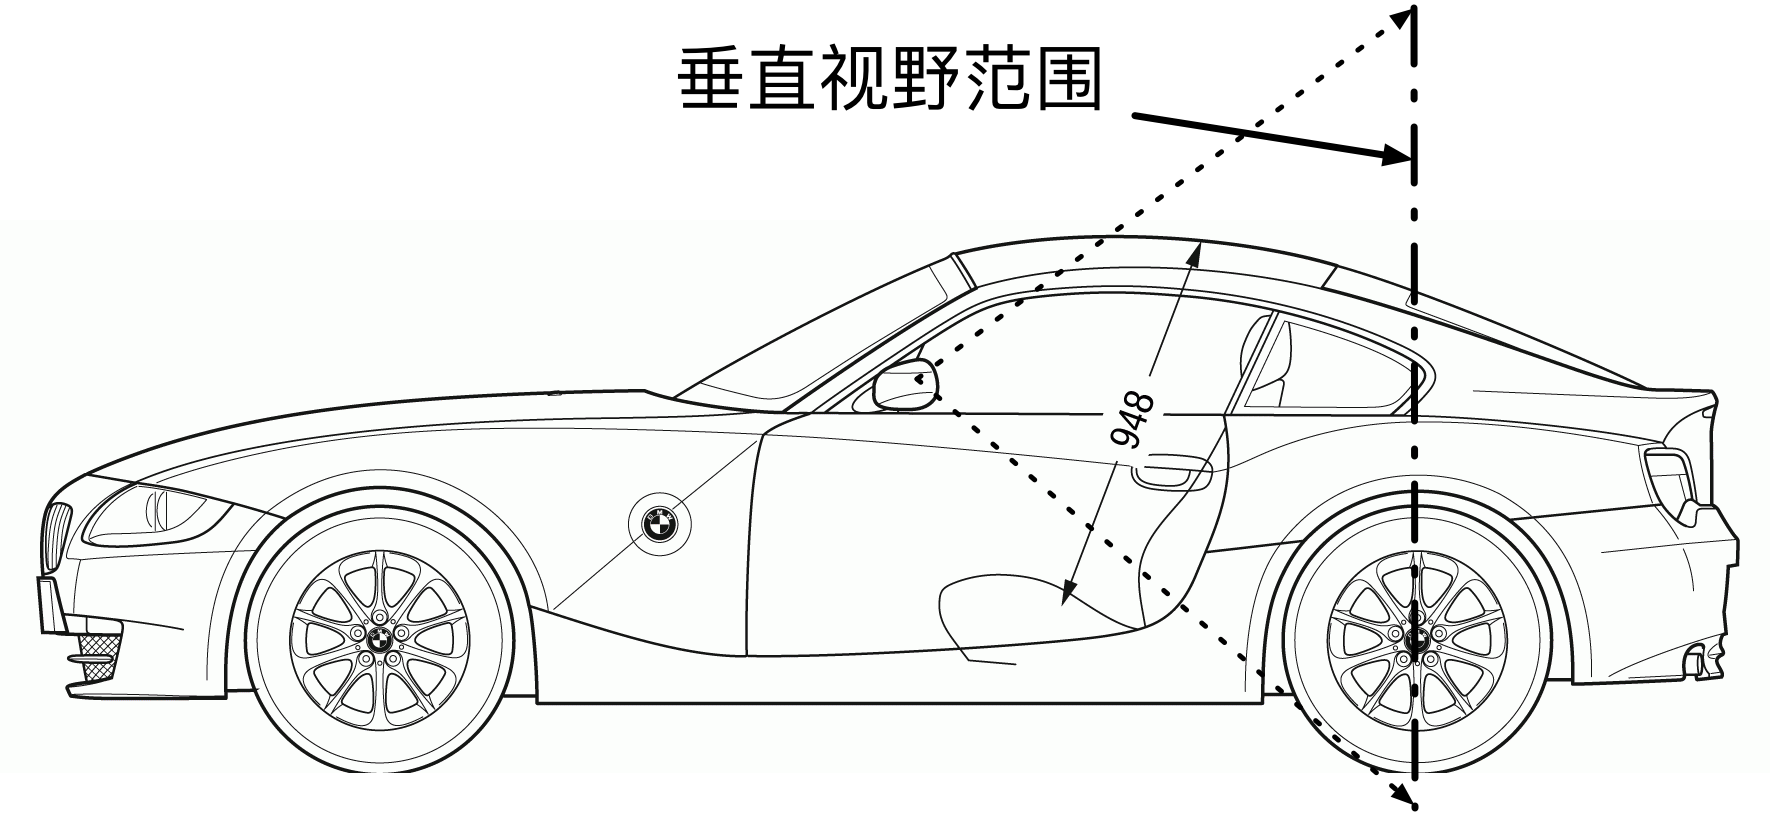
\includegraphics[width=12cm]{hight.png}
\caption{垂直视野范围的定义}
\label{hight}
\end{figure}

\subsection{畸变率模型}
\subsubsection{畸变率模型的建立}

\par 畸变率是衡量汽车后视镜是否合格的一个重要的技术指标,我们提出畸变率衡量指标,以便分析和对照。

\par 将镜面放置于$XOZ$平面,并作平行于坐标轴$50 \times 50$的网络划分,选取各个网格点与眼点的连线,作为入射光线,由反射定律得到反射光线,在平行于$XOZ$平面的面$(y>0)$处设置无限大光屏接收反射光线,得到对应的$50 \times 50$的网格点。
\par 对镜面上$50 \times 50$的所有网格点对间的距离求和:

\begin{equation}
	\sum\limits_{i = 1}^{50}\sum\limits_{j = i + 1}^{50} D_{ij}
\end{equation} 

\par 对接收光屏上$50 \times 50$的所有网格点对间的距离求和:

\begin{equation}
	\sum\limits_{i = 1}^{50}\sum\limits_{j = i + 1}^{50} d_{ij}
\end{equation}

\par 随着接收光屏与镜面间的距离增大,接收屏上的网格点间距同比增大,但是对于可看到的图像的外形没有影响,因此建立相似比系数来消除图像放大对格点间距离的影响。
\par 我们将相似比定义为镜面上$50 \times 50$的格点构成的区域最长边长与接收屏上$50 \times 50$的格点构成的区域最长边长的比值$\beta$。

\begin{equation}
	\beta = \frac{L_{\mathop{max}}}{l_{\mathop{max}}} \times 100 \%
\end{equation}

\par 畸变率$\alpha$定义如下公式(\ref{畸变率})所示:


\begin{equation}
\label{畸变率}
	\alpha = \frac{\mid \beta \sum\limits_{i = 1}^{50}\sum\limits_{j = i + 1}^{50} d_{ij} - \sum\limits_{i = 1}^{50}\sum\limits_{j = i + 1}^{50} D_{ij} \mid}{\sum\limits_{i = 1}^{50}\sum\limits_{j = i + 1}^{50} D_{ij}} \times 100 \%
\end{equation}

\subsubsection{畸变率模型的验证}

\par 按照定义计算得到平面镜的畸变率为$4.32402\times 10^{-12}\%$,可以确定在不存在畸变时,模型计算结果约为0。


\subsection{综合评价指标$K$}
\par 建立综合评价指标$K$,描述畸变率和视野范围的综合优化结果。计算方法如下公式(\ref{K})所示(其中L表示水平视野宽度):
\begin{equation}
\label{K}
	K = (1 - \alpha) \cdot L
\end{equation}

\subsection{镜面模型}
\subsubsection{镜面模型坐标}

\par 对于镜面模型的建立。确定如下图(\ref{basic})所示的坐标系:

\begin{figure}[!htb]
\centering
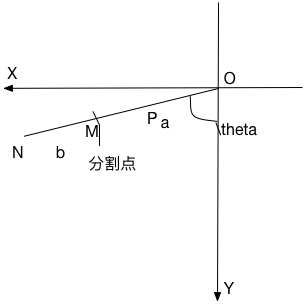
\includegraphics[width=8cm]{basic.png}
\caption{镜面坐标系建立}
\label{basic}
\end{figure}


\subsubsection{镜面模型方案一}

\begin{figure}[!htbp]  
\begin{minipage}[t]{0.5\textwidth}
\centering  
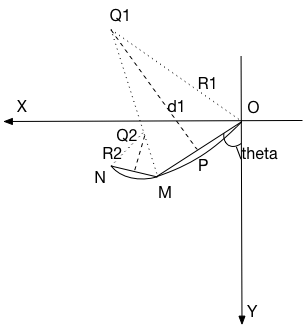
\includegraphics[width=\linewidth]{plan1.png} \\
\caption{方案一镜面设计(坐标)} \label{plan1}
\end{minipage}
\hspace{1ex}
\begin{minipage}[t]{0.5\textwidth}  
\centering  
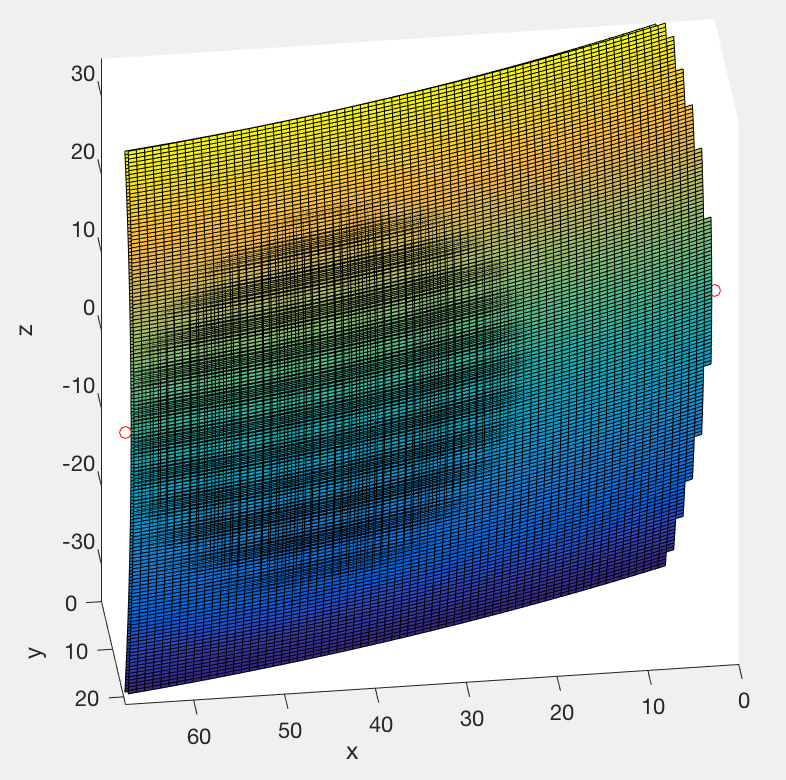
\includegraphics[width=\linewidth]{plan1-0.png}\\
\caption{方案一镜面设计(图像)}  \label{plan1-0}
\end{minipage}  
\end{figure} 


\par 假设左侧外后视镜的水平中线在$XOY$平面内,图(\ref{plan1})为后视镜的在$XOY$平面内的截面。后视镜由两个曲率不同的球面镜组成,两球面在$XOY$平面上的截面的弧线分别为弧$OM$、弧$MN$。

\par 定义$OM = a$, $MN = b$, $a + b = length$, $\frac{b}{a} = cutRatio$,设$Q_1$点的坐标为$(x_1,y_1,0)$,在$XOY$平面上$Q_1$点的坐标为$(x_1,y_1)$ 为镜面截线与$y$轴的夹角。

\par 镜面与$XOY$平面的交线的直线方程可以抽象为公式(\ref{镜面与$XOY$平面的交线的直线方程}):
 
\begin{equation}
\label{镜面与$XOY$平面的交线的直线方程}
	y = \mathop{cot}\theta \cdot x
\end{equation}

$Q_1$点到镜面的距离$d_1$(\ref{d1})即为$Q_1$点到直线$OM$的距离,通过点到直线的距离公式得:

\begin{equation}
\label{d1}
	d_1 = \frac{\mid \mathop{cot}\theta \cdot x_1 + y_1 \mid}{\sqrt{\mathop{cot}^{2} \theta + 1}} 
\end{equation}

\par 对直角三角形$Q_1OP$由勾股定理可得:$ d_1^2 + \left( \frac{a}{2} \right) = R_1^2$,将$d_1$带入得公式(\ref{plan1dis1}):
\begin{equation}
\label{plan1dis1}
	\left( \frac{\mid \mathop{cot}\theta \cdot x_1 + y_1 \mid}{\sqrt{\mathop{cot}^{2} \theta + 1}} \right)^2 +\left( \frac{a}{2} \right) = R_1^2
\end{equation}

\par 由设计可得$P$点坐标为:$P(\frac{a}{2} \mathop{sin} \theta, \frac{a}{2} \mathop{cos} \theta)$

\par 由中垂线定理、$Q_1P$与镜面垂直(即两直线垂直),斜率之积为$-1$得公式(\ref{plan1-1}):

\begin{equation}
\label{plan1-1}
	\frac{y_1 - \frac{a}{2} \mathop{cos} \theta}{x_1 - \frac{a}{2} \mathop{sin} \theta} \cdot \mathop{cot}\theta = -1
\end{equation}

\par (\ref{plan1dis1})(\ref{plan1-1})两式联立可解得:$Q_1(x_1,y_1)$,在空间中大曲率半径镜面的球心坐标为 $Q_1(x_1,y_1,0)$。由设计可知$M$点坐标为$M(a \mathop{sin} \theta, a \mathop{cos} \theta)$,则在二维平面$XOY$内,$Q_1M$的斜率为:

$$k = \frac{y_1 - a \mathop{cos} \theta}{x_1 - a \mathop{sin} \theta}$$
 
\par 可以得到$Q_1M$的直线方程为:
\begin{equation}
\label{plan1-q1m}
	y = \frac{y_1 - a \mathop{cos} \theta}{x_1 - a \mathop{sin} \theta} (x - a \mathop{sin} \theta ) + a \mathop{cos} \theta
\end{equation}

在本设计下,$Q_2$点在直线$Q_1M$上,设$Q_2$点的坐标为$Q_2(x_2, y_2)$,$Q_2$和$M$两点间的距离为小曲律半径镜面的半径$R_2$

\begin{equation}
\label{plan1-r2}
	\sqrt{(x_2 - a \mathop{sin}\theta )^2 + (y_2 - a \mathop{cos}\theta )^2} = R_2
\end{equation}
\par 将坐标代入公式(\ref{plan1-q1m})后与公式(\ref{plan1-r2})联立可解得球心坐标$Q_2(x_2,y_2)$,则在空间中小曲率半径镜面的球心坐标为$Q_2(x_2,y_2,0)$。


\subsubsection{镜面模型方案二}

\par 方案二基于$MNO$三点共线设计,且与方案一使用相同变量名和坐标系,图(\ref{plan2})为后视镜的在$XOY$平面内的截面。


\begin{figure}[!htbp]  
\begin{minipage}[t]{0.5\textwidth}
\centering  
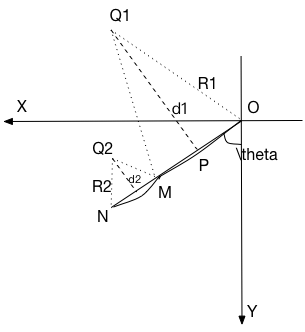
\includegraphics[width=\linewidth]{plan2.png} \\
\caption{方案二镜面设计(坐标)} \label{plan2}
\end{minipage}
\hspace{1ex}
\begin{minipage}[t]{0.5\textwidth}  
\centering  
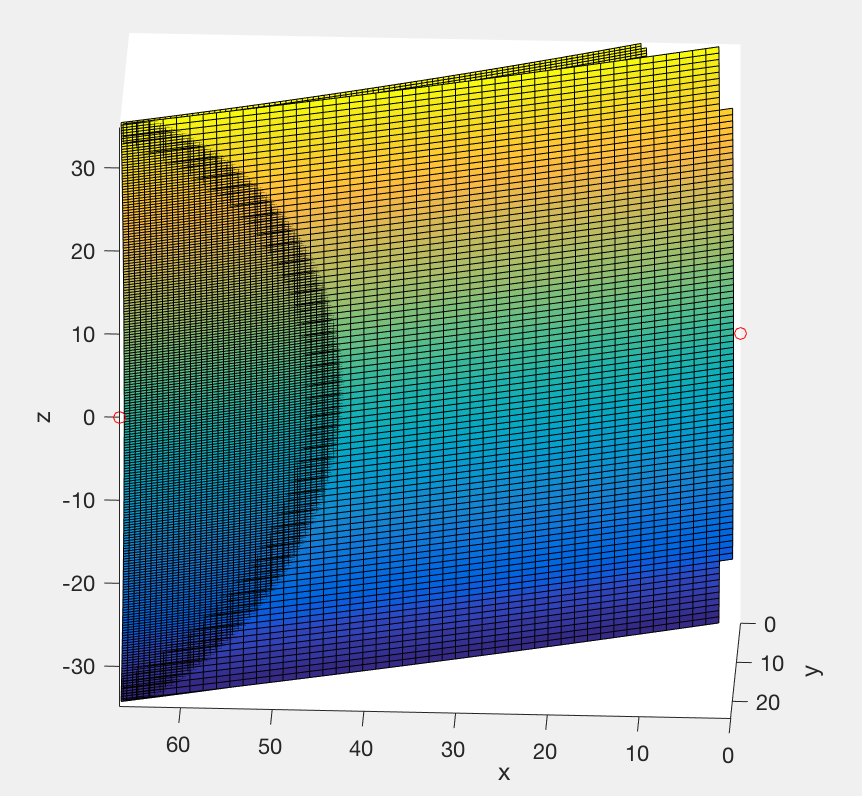
\includegraphics[width=\linewidth]{plan2-0.png}\\
\caption{方案二镜面设计(图像)}  \label{plan2-0}
\end{minipage}  
\end{figure} 

\par 对于大曲率半径镜面的球心$Q_1$的设计与方案一相同,对于小曲率半径镜面的球心$Q_2(x_2,y_2)$,有距离$d_2$:

\begin{equation}
	d_2 = \frac{\mid \mathop{cot}\theta \cdot x_2 + y_2 \mid}{\sqrt{\mathop{cot}^{2} \theta + 1}} 
\end{equation}
\par 对直角三角形$Q_2NM$由勾股定理可得:$d_2^2 + \left( \frac{b}{2} \right) = R_2^2$,将$d_1$代入得公式(\ref{plan2-dis}):

\begin{equation}
\label{plan2-dis}
	\frac{\mid \mathop{cot}\theta \cdot x_2 + y_2 \mid}{\sqrt{\mathop{cot}^{2} \theta + 1}} = \sqrt{R_2^2 - \left( \frac{b}{2} \right)^2} 	
\end{equation}
\par 与方案一同理得公式(\ref{plan2-1}):
\begin{equation}
\label{plan2-1}
	\frac{\left(a + \frac{b}{2}\right) \mathop{cos} \theta - y_2}{\left( a+ \frac{b}{2} \right) \mathop{sin} \theta - x_2} \cdot \mathop{cot}\theta = -1
\end{equation}
\par 联立公式(\ref{plan2-dis})(\ref{plan2-1})解得球心坐标$Q_2(x_2,y_2)$,则在空间中小曲率半径镜面的球心坐标为$Q_2(x_2,y_2,0)$。

\section{模型求解}

\subsection{问题一求解}

\subsubsection{镜面尺寸的确定}
\par $M$类是至少有4个车轮并且用于载客的机动车辆;$M_1$类是包括驾驶员座位在内,座位数不超过9座的载客车。因此本文针对的典型的小型家用轿车属于$M_1$类。根据国家标准$GB 15084-94$中关于后视镜最小尺寸要求标准(如表(\ref{后视镜最小尺寸要求标准})所示)。本文所设计后视镜属于第三类后视镜,且其反射面的曲率半径不得小于$1200mm$。考虑制造公差,反射面曲率半径一般设定在$1260mm$\upcite{后视镜设计} 。

\begin{table}[!htbp]
\centering
\caption{后视镜最小尺寸要求标准}
\label{后视镜最小尺寸要求标准}
\begin{tabular}{cccc}
\toprule
后视镜类别 & 适用汽车类型 & $a$ & $b$	\\ \midrule
 II	 & $M_2$ 、$M_3$ 和$N_2$、 $N_3$ &  $a =  \frac{170}{1+\frac{1000}{r}}$& 200\\ 
III & $M_1$ 和$N_1$& $a =  \frac{130}{1+\frac{1000}{r}}$&  70\\ 
\bottomrule 
\end{tabular}
\end{table}

\par 根据国家标准确定最小设计参数:$b \geqslant 70mm$,$r \geqslant 1200mm$(如图\ref{fig:后视镜最小尺寸示意}所示)。本文中主视野区最小参数$a$:
$$a \geqslant \frac{130}{1+\frac{1000}{1260}} = 72.48$$

\par 本文首先按照最小尺寸进行设计,之后参照主流量产车平均设计尺寸进行等比放大。
\begin{figure}[h]
\small
\centering
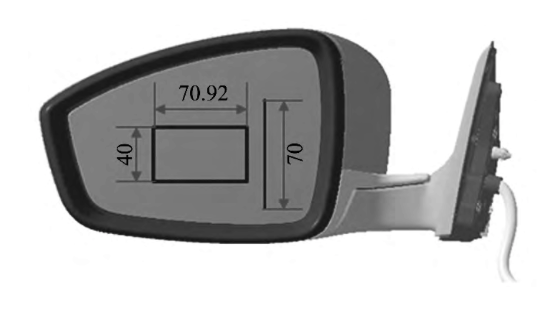
\includegraphics[width=12cm]{minsize.png}
\caption{国标中后视镜最小尺寸示意} \label{fig:后视镜最小尺寸示意}
\end{figure}

\par 放大后外后视镜镜片参数为:
$length = 72.48\times 2.72 = 197.1456$,            
$width = 70 \times 1.625 = 113.75$。(实际生产时切割出所需要的形状)

\subsubsection{畸变率的求解}

\par 通过方案一、方案二模型得到待定系数的镜面。以第一种方案为例:
\par 曲率半径较小的球面从$y$轴正方向看落在$XOZ$平面上的半径rr:

\begin{equation}
	\mathop{rr} = length \times \frac{cutRatio}{2}
\end{equation}

\par 外后视镜镜面上点的$y$坐标$f$:
\begin{equation}
	f = 
	\begin{cases}
		\sqrt{R_1^2 - (x-x_1)^2 - (z - z_1)^2} + y_1\quad \quad otherwise
		\\
		\sqrt{R_2^2 - (x-x_2)^2 - (z - z_2)^2} + y_2 \quad \quad 
		\sqrt{(x-x_2)^2 - (z - z_2)^2} < \mathop{rr} 
	\end{cases} 
\end{equation}

\par 通过实际测量数据确定的驾驶员双眼中点坐标$(X_0,Y_0,Z_0)$(单位mm):

\begin{equation}
	\begin{cases}
		X_0 = -450 \\ 
		Y_0 = 730 \\
		Z_0 = 0 
	\end{cases} 
\end{equation}
\par 已知曲面方程和曲面上一个固定点,通过公式(\ref{F})求得该点的切平面方程(公式(\ref{qiepingmian}))、法线方程(公式(\ref{faxian}))、法向量(公式(\ref{faxiangliang}))。
\begin{equation}
\label{F}
	\begin{cases}
		F_1 = f_x = diff(f,x) \\
		F_2 = f_z = diff(f,z) \\
		F_3 = f_y = -1
	\end{cases}
\end{equation}

\begin{equation}
\label{qiepingmian}
	(x - x_0)F_1(x_0,y_0,z_0) + (y - y_0)F_2(x_0,y_0,z_0) + (z - z_0)F_3(x_0,y_0,z_0) = 0
\end{equation}

\begin{equation}
\label{faxian}
	\frac{x - x_0}{F_1(x_0,y_0,z_0)} = \frac{y - y_0}{F_2(x_0,y_0,z_0)} = \frac{z - z_0}{F_3(x_0,y_0,z_0)} 
\end{equation}

\begin{equation}
\label{faxiangliang}
	\vec{n_0} = \left[\frac{F_1}{\sqrt{F_1^2+F_2^2+F_3^2}},\quad \frac{F_2}{\sqrt{F_1^2+F_2^2+F_3^2}},\quad \frac{F_3}{\sqrt{F_1^2+F_2^2+F_3^2}}\right]
\end{equation}
\par 给定入射光线方向向量$\vec{a}$:
\begin{equation}
	\vec{a} = [x - X_0,\quad f - Y_0, \quad z - Z_0 ]
\end{equation}
\par 通过公式(\ref{guiyi})将归一化,代入公式(\ref{b})中求得反射光线与光屏的交点坐标$(X_x,Y_y,Z_z)$(如公示(\ref{jiaodian})所示,其中dis为光屏与外后视镜的距离)。
\begin{equation}
\label{guiyi}
	\vec{a} = \frac{\vec{a}}{\|\vec{a}\|}   
\end{equation}

\begin{equation}
\label{b}
	\vec{b} = \vec{a} - 2 \cdot (\vec{a} \cdot \vec{n_0}) \cdot \vec{n_0}
\end{equation}

\begin{equation}
\label{jiaodian}
	\begin{cases}
		X_x = \frac{Y_y - Y}{b_y \cdot b_x} + X \\
		Y_y = dis \\
		Z_z = \frac{Y_y - Y}{b_y \cdot b_x} + Z
	\end{cases}
\end{equation}

\par 将外后视镜镜面以及光屏上对应点的数据代入公式(\ref{畸变率})中求解得到外后视镜的畸变率$\alpha$。

\subsubsection{视野范围的求解}
\begin{enumerate}
	\item 按照畸变率计算中的方法在外后视镜面上完成$50\times50$的投点。
	\item 与求畸变率不同,视野求解需要考虑左右眼的差距,此时眼点位置依据国家标准,在畸变率计算中确定的驾驶员坐标的基础上,水平增减$32.5mm$作为左右眼点的坐标。
	\item 对于水平视野范围计算,左后视镜:将屏放在10m的位置,分别计算左右眼水平视野最大宽度,综合取最大值。右后视镜时:将屏放在20m的位置,分别计算左右眼水平视野最大宽度,综合取最大值。
	\item 对于垂直视野范围计算,将光屏放置在汽车后轴的位置(按照常见量产车平均轴距确定),测量垂直方向上的最大视野范围。
	\item 剩下步骤与计算畸变率一致。
\end{enumerate}

\subsubsection{综合求解结果}
通过上述方法进行求解后得到如下表(\ref{计算结果1})所示的最终结果(单位为mm),在方案一与方案二中,我们优先选择了方案一。
\begin{table}[!htbp]
\centering
\caption{计算结果}
\label{计算结果1}
\begin{tabular}{cccccc}
\toprule
方法类别 & cutRatio & $R_2$ & $\alpha$(畸变率) & $L$(水平视野范围) & $K$(综合指标) \\ \midrule

方案一左侧 &0.5 &    500   &     3.86294128731591\%          &5527.28149862427  &    5313.76585954774 \\
方案一右侧 & 0.2 &   500    &     11.4355762806068\%          &11536.1656322035   & 10216.9386114758 \\
方案二左侧 &0.2 &    500     &          4.2228727\%          & 3502.4475909647     &  3354.54368781404 \\                                                  
方案二右侧 & 0.2    & 500      &   11.4355762806068\%           & 9755.34371439532  &     8639.76394250026 \\       
\bottomrule 
\end{tabular}
\end{table}

\par 如图(\ref{fig:DD1Z})所示为最终方案左侧外后视镜在10米处可观察到的视野范围(后视镜中线以上)。
\begin{figure}[!htbp]
\small
\centering
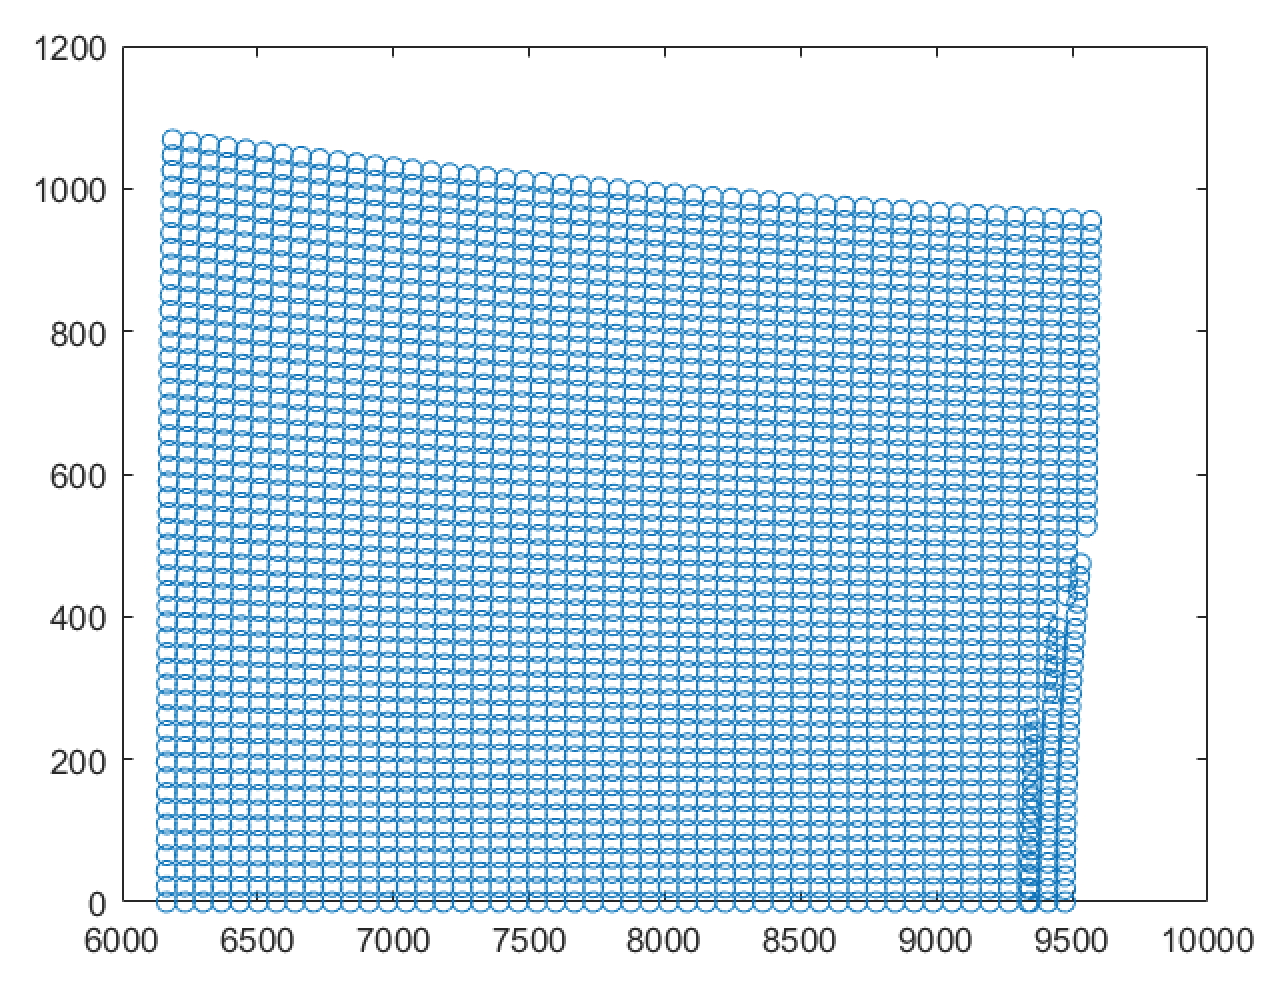
\includegraphics[width=12cm]{DD1Z.png}
\caption{左侧后视镜中线以上视野范围} \label{fig:DD1Z}
\end{figure}

\par 如图(\ref{fig:DD1Y})所示为最终方案右侧外后视镜在20米处可观察到的视野范围(后视镜中线以上)。

\begin{figure}[!htbp]
\small
\centering
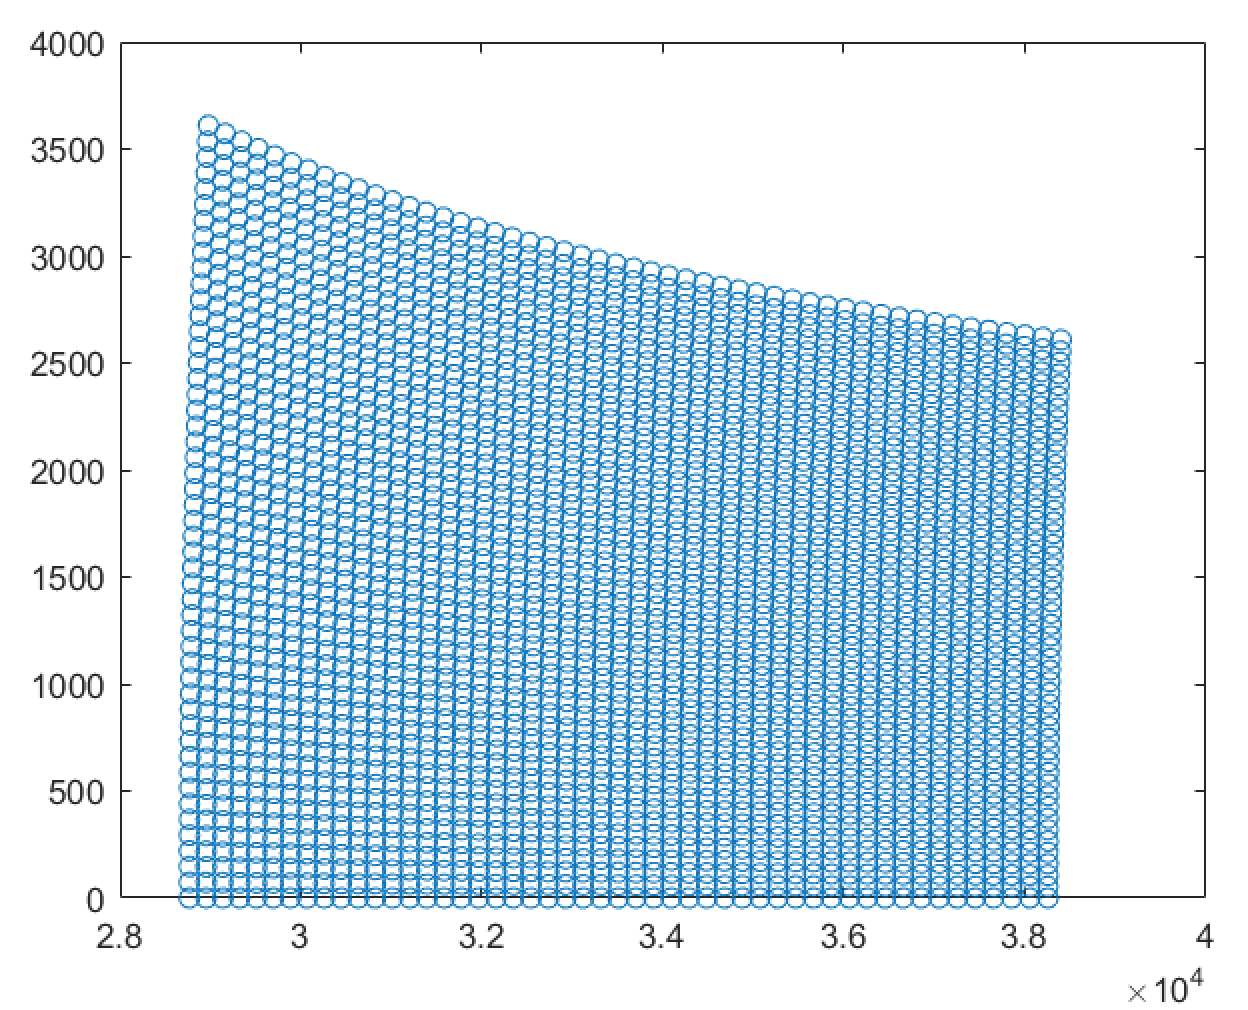
\includegraphics[width=12cm]{DD1Y.png}
\caption{右侧后视镜中线以上视野范围} \label{fig:DD1Y}
\end{figure}

 
\subsubsection{外后视镜角度调整}
\par 由后视镜安装的初始位置一般难以符合视野的要求,所以必须将其调整到合适位置,使其视野能涵盖国标规定的区域。因此在安装时能对外后视镜片进行绕坐标轴的旋转。

\par 通过调整外后视镜的安装角度,可使得外后视镜视野范围覆盖国标要求的区域以及汽车后轮等区域。
 
\subsection{问题二求解}
\subsubsection{求解方法}
\par 针对第二问,本文给出了一种方便司机简单易行的快速判断镜中物体的距离与方位的方法并进行误差分析。
\par 根据第1问,可以通过外后视镜上的点、人眼以及光屏的位置确定光屏上的点。因而若已知外后视镜中物体的一段长度,且人眼的位置固定,则可以通过改变光屏距离外后视镜的距离来计算原物体的长度。在行车中,该原物体通常是车辆,本文将车辆为例给出简易判断方法。
\par 通过查询资料,得到量产车辆的一般宽度(车身外侧钣金最突点之间的距离)为$W=1700mm$,将第一问原来均匀投在一个面上的点,改为投在一条线段的两个端点处即可,来模拟车宽在外后视镜的镜像长度。本文中以外后视镜水平线为基准来设置线段。通过改变车距(即屏距离外后视镜的距离),和该水平线段的长度,可以得到原物体的宽度,最终通过种模拟找到水平线段长度。确定原物体的宽度为平均车宽$W$时的车距。
\par 结合实际情况,本文以水平线段长度占外后视镜长度的比例给出。由于双曲率后视镜两种不同曲率下图像畸变存在明显差异,分水平线段在分界线以左(如图(\ref{q2-2})所示)以右(如图(\ref{q2-1})所示)两种情况讨论。

\begin{figure}[!htbp]  
\begin{minipage}[t]{0.5\textwidth}
\centering  
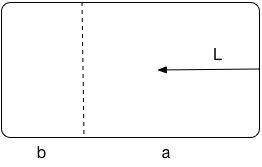
\includegraphics[width=\linewidth]{q2-1.png} \\
\caption{水平线段在分界线以右} \label{q2-1}
\end{minipage}
\hspace{1ex}
\begin{minipage}[t]{0.5\textwidth}  
\centering  
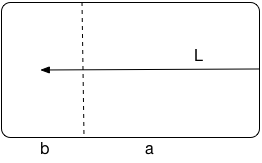
\includegraphics[width=\linewidth]{q2-2.png}\\
\caption{水平线段在分界线以左}  \label{q2-2}
\end{minipage}  
\end{figure} 


\par 判断方法实际给出的形式是:水平线段在分界线以左或以右,长度比例为$rate$时车距为$n$米。联系实际,车距采用米为最小单位,因而会引入误差。当车距为确定整数米时,计算得到的实际车宽在1700mm左右一定范围内波动从而产生误差。

\subsubsection{综合求解结果}

通过程序模拟,我们得到如下结果。

\begin{table}[!htbp]
\centering
\caption{左后视镜b区}
\label{左后视镜b区}
\begin{tabular}{cccc}
\toprule
 $rate$左边占比(已占据a区域)  &  距后视镜距离(m) &  $W$车宽(mm) &  $\Delta E$相对误差  \\ \midrule
$\frac{1}{4}$ & 8 & 1782 & 4.82\% \\
$\frac{1}{3}$ & 7 & 1677 & 1.35\% \\
$\frac{1}{2}$ & 6 & 1635 & 3.82\% \\
\bottomrule 
\end{tabular}
\end{table}

\begin{table}[!htbp]
\centering
\caption{左后视镜a区}
\label{左后视镜a区}
\begin{tabular}{cccc}
\toprule
$rate$左边占比 & 距后视镜距离(m) & $W$车宽(mm) & $\Delta E$相对误差  \\ \midrule
$\frac{1}{4}$ & 40 & 1679 & 1.23\% \\
$\frac{1}{3}$ & 30 & 1688 & 0.71\% \\
$\frac{1}{2}$ & 20 & 1707 & 0.41\% \\
\bottomrule 
\end{tabular}
\end{table}

\begin{table}[!htbp]
\centering
\caption{右后视镜b区}
\label{右后视镜b区}
\begin{tabular}{cccc}
\toprule
$rate$右边占比(已占据a区域)& 距后视镜距离(m) & $W$车宽(mm) & $\Delta E$相对误差  \\ \midrule
$\frac{1}{4}$ & 4 & 1831 & 7.71\% \\
$\frac{1}{3}$ & 4 & 1868 & 9.88\% \\
$\frac{1}{2}$ & 3 & 1456 & 14.35\% \\
\bottomrule 
\end{tabular}
\end{table}

\begin{table}[!htbp]
\centering
\caption{右后视镜a区}
\label{右后视镜a区}
\begin{tabular}{cccc}
\toprule
$rate$右边占比 & 距后视镜距离(m) & $W$车宽(mm) & $\Delta E$相对误差  \\ \midrule
$\frac{1}{4}$ & 16 & 1665 & 2.06\% \\
$\frac{1}{3}$ & 12 & 1672 & 1.59\% \\
$\frac{1}{2}$ & 8 & 1687 & 0.76\% \\
\bottomrule 
\end{tabular}
\end{table}

\par 驾驶员可按照上表(\ref{左后视镜b区},\ref{左后视镜a区},\ref{右后视镜b区},\ref{右后视镜a区})通过在后视镜中宽度的占比大致确定后车距离。

\subsection{问题三求解}
\par 在问题三中,我们选取量产车:奇瑞QQ 2013款(如图(\ref{fig:qq3})所示),通过本文建立的模型测算其外后视镜视野范围、图像畸变率等参数。该车原外后视镜尺寸为$165mm \times 126mm$ 曲率半径为$1200mm$。
\begin{figure}[h]
\small
\centering
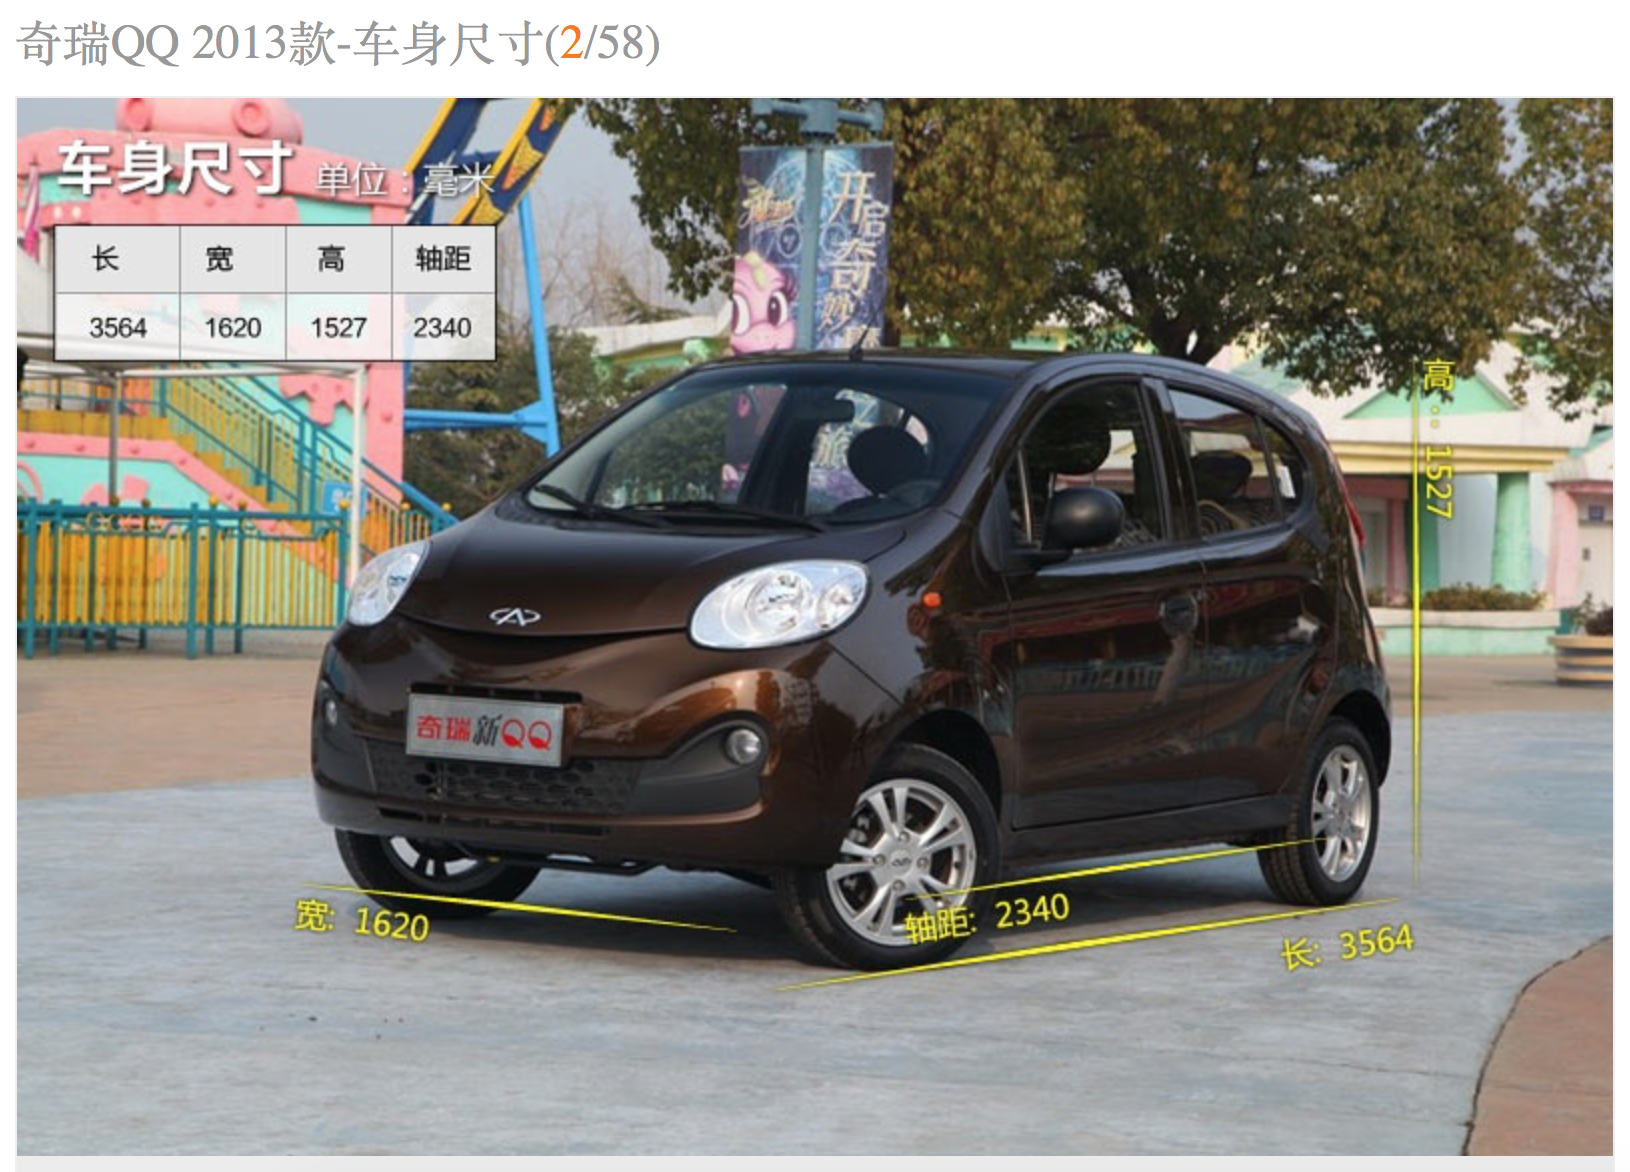
\includegraphics[width=12cm]{qq3.png}
\caption{奇瑞QQ 2013款外形尺寸图} \label{fig:qq3}
\end{figure}

计算得原后视镜相关参数如下表(\ref{原车后视镜计算数据})所示:
\begin{table}[!htbp]
\centering
\caption{原车后视镜计算数据}
\label{原车后视镜计算数据}
\begin{tabular}{|c|c|c|}
\toprule
左后视镜视野范围(mm)$L$ & 左后视镜畸变率$\alpha$ & 左后视综合指标$K$ \\ \hline 
4553.20823986563 & 2.88920268960021\%  & 4421.65682493633 \\ \hline 


右后视镜视野范围(mm)$L$ & 右后视镜畸变率$\alpha$  & 右后视综合指标$K$ \\ \hline
7997.14730406906 & 10.2758921450585\%  &  7175.36907242147 \\

\bottomrule 
\end{tabular}

\end{table}
\par 如图(\ref{fig:qiruiz},\ref{fig:qiruiy})所示分别为原车后视镜的外后视镜中线以上视野范围。

\begin{figure}[!htpb]
\small
\centering
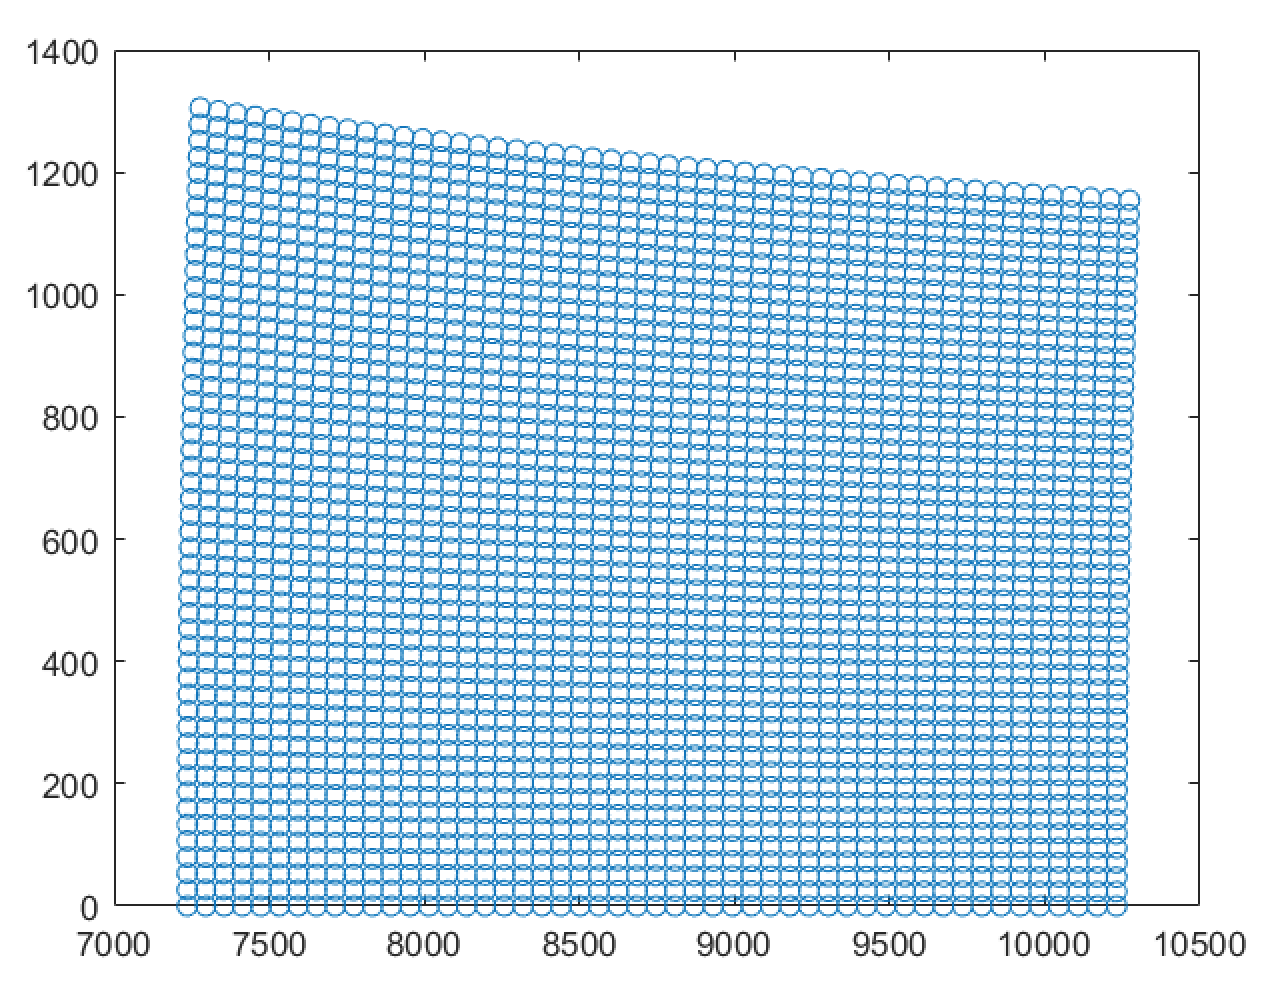
\includegraphics[width=12cm]{qiruiz.png}
\caption{原车左侧后视镜视野范围(中线以上)} \label{fig:qiruiz}
\end{figure}

\begin{figure}[!htpb]
\small
\centering
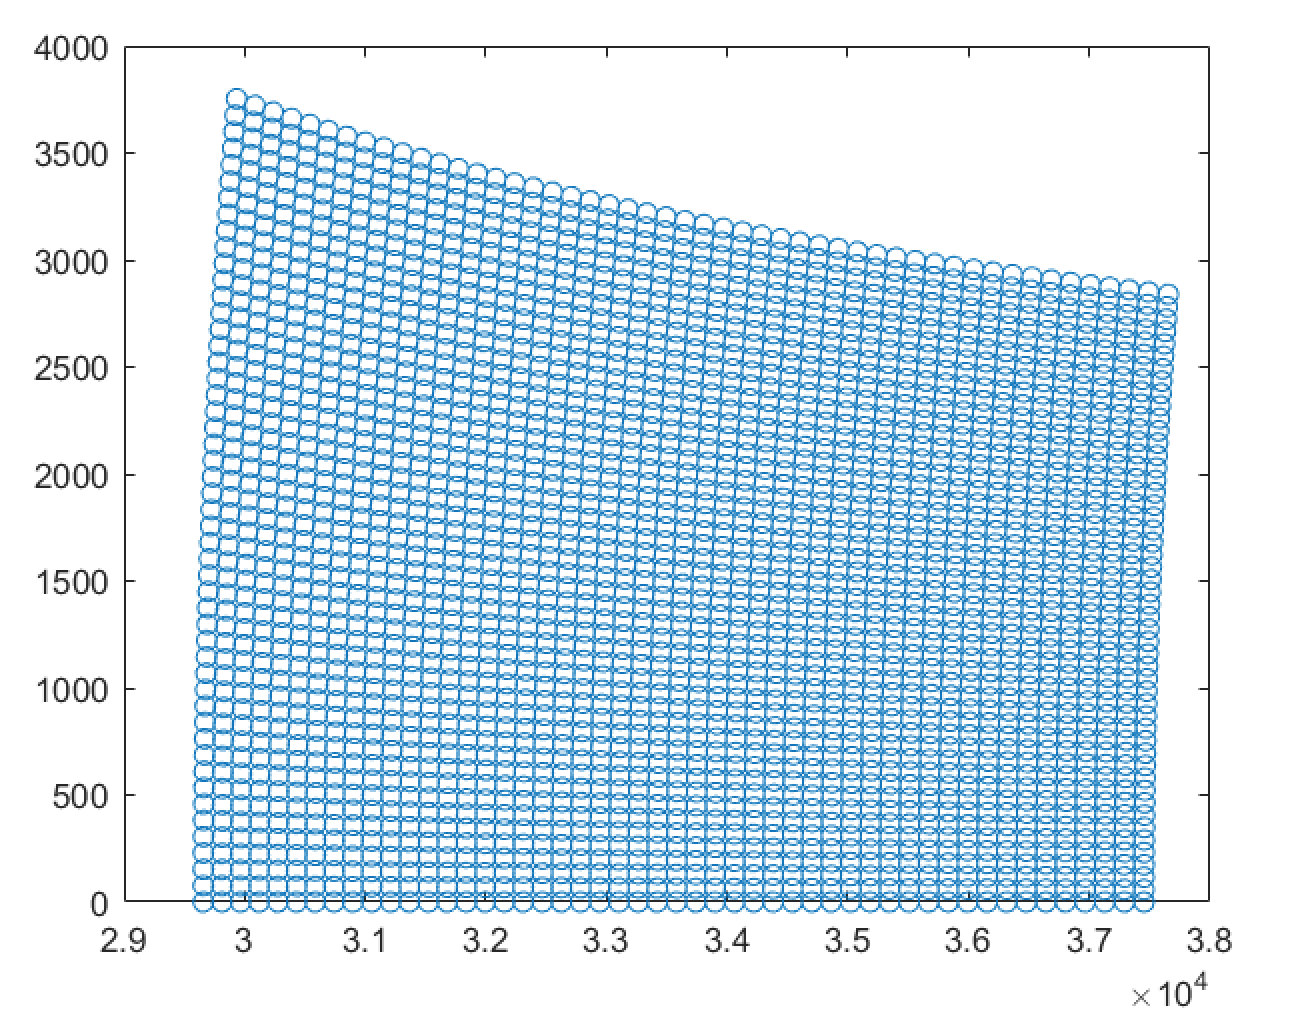
\includegraphics[width=12cm]{qiruiyou.png}
\caption{原车右侧后视镜视野范围(中线以上)} \label{fig:qiruiy}
\end{figure}

\par 同时我们设计的双曲率后视镜采取曲率半径分别为$1260mm$与$500mm$,得到驾驶员的左侧视野范围为$5527mm$,畸变率为$3.8\%$;右侧的视野范围为$11536 mm$,畸变率为$11.4\%$。

\par 本文设计的外后视镜模型在畸变率基本没变的基础上将左右两侧的视野范围大大增加,因此我们的设计更优于原车设计。


\section{模型优缺点}
\subsection{模型优点}
\begin{enumerate}
	\item 畸变率模型创新性地提出了凸面镜图像畸变率的定量化刻画方法,并且该指标经检验是合理的。
	\item 双曲率外后视镜是市场上最流行的设计,并且本文设计的双曲率外后视镜,很好的符合了国家标准,并尽可能在保证失真率可控的前提下提高了后视镜视野范围。
	\item 双曲率外后视镜设计是依据车型、驾驶员眼点位置与后视镜相对位置、视野要求三个要素,运用光学原理和计算机模拟方法,对车辆的左右不同视野角度选择不同的曲率半径。在失真率可接受的条件下实现扩大视野、减少盲区的目的。
\end{enumerate}
\subsection{模型缺点}
\begin{enumerate}
	\item 外后视镜模型没有考虑双曲率球面在拼接过程中的边缘的平滑过渡问题。
	\item 在畸变率模型中,算法的复杂度高,计算耗时长。
\end{enumerate}
\section{模型改进方向}
\begin{enumerate}
	\item 在构造外后视镜模型的时候,选取不同的曲率半径的两种球面拼接而成,在改进工作中,需要考虑用一般的二次曲面来构造外后视镜。该方法能构造出变曲率外后视镜,并且不需要考虑镜面区域的过渡区域的问题。
	\item 本文设计的畸变率的计算模型,复杂度比较高,在计算机求解过程中,运算时间比较长,在改进过程中建立实际图像与后视镜反射后的图像的重叠程度作为畸变率模型的新指标。
\end{enumerate}


%参考文献
\begin{thebibliography}{9}%宽度9
 \bibitem{大视野后视镜} 王卫华. 汽车大视野后视镜的理论建模与应用技术研究[D]. 武汉理工大学, 2006.
 \bibitem{后视镜设计} 周博. 汽车外后视镜镜片尺寸及位置设计[J]. 上海汽车, 2015(12):41-44.
 \bibitem{后视镜仿真} 牛慧超. 汽车后视镜检测系统的研究及仿真设计[D]. 武汉理工大学, 2009.
 \bibitem{汽车分类}\url{https://www.zybang.com/question/cf0e112815df2cd96348c0e973e0a546.html}
\end{thebibliography}

\newpage
%附录
\appendix

\section{附件内容}
\begin{enumerate}
	\item 计算中间数据.xlsx
	\item 程序.zip
\end{enumerate}



\end{document} 